% fig_loops_pr.tex -- generated by gen_fig_loops.py from ../theory/h2probe.txt; do not edit by hand.
\definecolor{fpV}{HTML}{D55E00}%
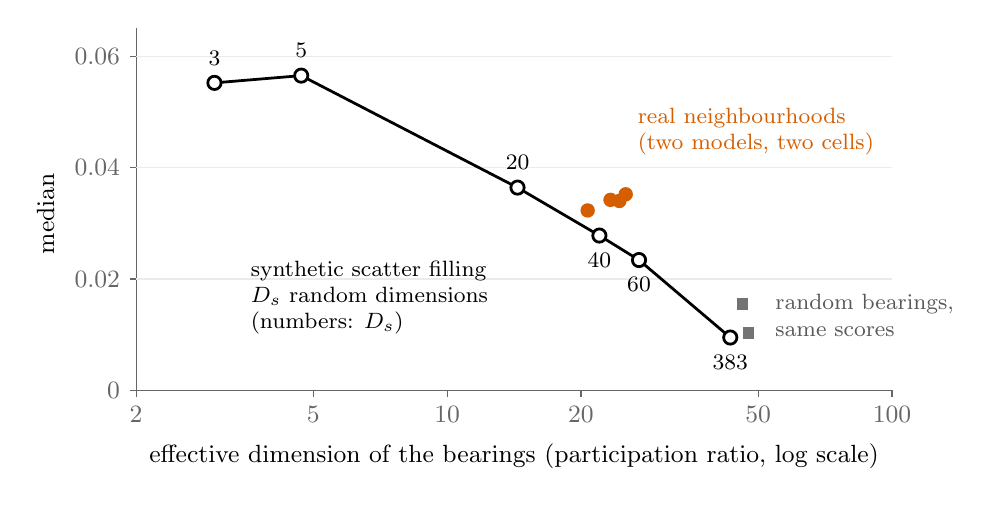
\begin{tikzpicture}[font=\small]
\draw[black!60] (0,0) -- (9.6,0); \draw[black!60] (0,0) -- (0,4.6);
\draw[black!60] (0.000,0) -- (0.000,-0.08) node[below] {2};
\draw[black!60] (2.249,0) -- (2.249,-0.08) node[below] {5};
\draw[black!60] (3.950,0) -- (3.950,-0.08) node[below] {10};
\draw[black!60] (5.650,0) -- (5.650,-0.08) node[below] {20};
\draw[black!60] (7.899,0) -- (7.899,-0.08) node[below] {50};
\draw[black!60] (9.600,0) -- (9.600,-0.08) node[below] {100};
\draw[black!60] (0,0.000) -- (-0.08,0.000) node[left] {0};
\draw[black!60] (0,1.415) -- (-0.08,1.415) node[left] {0.02};
\draw[black!8] (0,1.415) -- (9.6,1.415);
\draw[black!60] (0,2.831) -- (-0.08,2.831) node[left] {0.04};
\draw[black!8] (0,2.831) -- (9.6,2.831);
\draw[black!60] (0,4.246) -- (-0.08,4.246) node[left] {0.06};
\draw[black!8] (0,4.246) -- (9.6,4.246);
\node[below] at (4.8,-0.55) {effective dimension of the bearings (participation ratio, log scale)};
\node[rotate=90] at (-1.15,2.3) {median $\LTmax$};
\draw[black, line width=1pt] (0.995,3.906) -- (2.097,3.998) -- (4.844,2.576) -- (5.884,1.967) -- (6.387,1.656) -- (7.546,0.672);
\filldraw[fill=white, draw=black, line width=1pt] (0.995,3.906) circle (2.4pt);
\node[font=\footnotesize, anchor=south] at (0.995,4.006) {$3$};
\filldraw[fill=white, draw=black, line width=1pt] (2.097,3.998) circle (2.4pt);
\node[font=\footnotesize, anchor=south] at (2.097,4.098) {$5$};
\filldraw[fill=white, draw=black, line width=1pt] (4.844,2.576) circle (2.4pt);
\node[font=\footnotesize, anchor=south] at (4.844,2.676) {$20$};
\filldraw[fill=white, draw=black, line width=1pt] (5.884,1.967) circle (2.4pt);
\node[font=\footnotesize, anchor=north] at (5.884,1.867) {$40$};
\filldraw[fill=white, draw=black, line width=1pt] (6.387,1.656) circle (2.4pt);
\node[font=\footnotesize, anchor=north] at (6.387,1.556) {$60$};
\filldraw[fill=white, draw=black, line width=1pt] (7.546,0.672) circle (2.4pt);
\node[font=\footnotesize, anchor=north] at (7.546,0.572) {$383$};
\fill[fpV] (5.735,2.286) circle (2.6pt);
\fill[black!55] (7.703,0.659) rectangle (7.843,0.799);
\fill[fpV] (6.218,2.491) circle (2.6pt);
\fill[black!55] (7.703,0.666) rectangle (7.843,0.806);
\fill[fpV] (6.025,2.420) circle (2.6pt);
\fill[black!55] (7.630,1.020) rectangle (7.770,1.160);
\fill[fpV] (6.138,2.406) circle (2.6pt);
\fill[black!55] (7.630,1.034) rectangle (7.770,1.174);
\node[fpV, anchor=south west, align=left, font=\footnotesize] at (6.247,2.866) {real neighbourhoods\\(two models, two cells)};
\node[black!65, anchor=west, align=left, font=\footnotesize] at (7.995,0.955) {random bearings,\\same scores};
\node[anchor=north east, align=left, font=\footnotesize] at (4.593,1.769) {synthetic scatter filling\\$D_s$ random dimensions\\(numbers: $D_s$)};
\end{tikzpicture}%
